

\section{Cборщик мусора JBGC}
\subsection{Введение}
Одним из самых популярных алгоритмов сборки мусора является  алгоритм маркировки и освобождения (англ. mark-and-sweep). Популярность обусловлена простотой, и тем, что данный алгоритм накладывает минимальные ограничения на язык сборщика мусора. Все этапы, необходимые для его построения представлены на рисунке 1.  Предлагаемая реализация сборщика мусора предусматривает возможность в дальнейшем реализовать и другие алгоритмы сборки мусора.  А причина, по которой был выбран именно данный алгоритм, как уже сказано ранее -- простота.


\begin{figure}[h!]
	\centering
	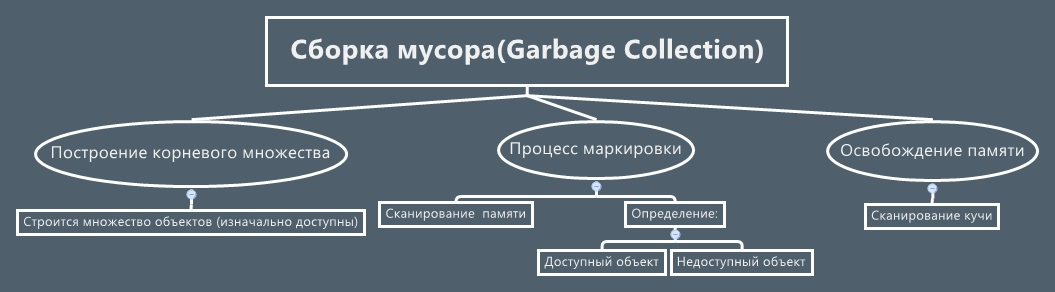
\includegraphics[width=500pt]{picture1.jpg}
	\caption{На схеме представлены три основных этапа сборки мусора}
	\centering
\end{figure}

Далее рассмотрим подробнее каждый из этапов в контексте сборщика мусора JBGC,  с которым можно самостоятельно ознакомиться.\footnote{URL: \url{https://github.com/danyaberezun/diploma/tree/master}} Реализация которого описана в \cite{realisation}.



\subsection{Процесс построения корневого множества и объектов кучи}
\subsubsection{Процесс построения корневого множества}
Данный процесс подробно рассмотрен в статье \cite{roots}.
При создании gc\_ptr, стоит учитывать то, что объекты могут создаваться как в куче, так и на стеке. Список стековых объектов  нужно обязательно хранить для того, чтобы уметь в дальнейшем отслеживать состояние объектов, сканировать объекты, начиная с рутов, и помечать мусор. 

Для того, чтобы отслеживать место создания объекта, заведен специальный флаг, который при вызове функции выделения памяти gc\_new  под gc\_ptr декларирует место создания объекта. Если флаг выставлен, значит объект создан в куче, если нет, на стеке.

Все ``умные указатели'' (gc\_ptr), вызывают в своем конструкторе функцию добавления себя в список корней, в случае загрузки стековой рамки на стек и функцию удаления себя из этого списка в своем диструкторе, в случае вытеснения стековой рамки. Статические объектами, являющиеся gc\_ptr, добавляются в список рутов в момент инициализации статической области. Все это происходит внутри класса gc\_ptr.


\subsubsection{Процесс построения метаинформации}
Модель представления объектов для сборки мусора была описана в \cite{meta}. Рассмотрим процесс построения метаинформации.

Когда выделяется память под объект в куче, перед ним кладется указатель на соответствующую ему метаинформацию. Ее нужно конструировать в случае, если при поиске в списке пар (typeid, classMeta), где classMeta -- список указателей на метаинформацию различных типов, не установлено соответствий. Если же поиск успешен, указатель на соответствующую типу метаинформацию вернет функция  поиска.

Процесс построения метаинформации включает в себя создание обертки объекта. Обертка создается в единственном экземпляре для каждого типа, создание происходит в gc\_new. Она хранит в себе смещения указателей вложенных объектов gc\_ptr относительно указателя на объект (это нужно для того, чтобы ходить по всем достижимым объектам). Все смещения записываются внутри функции gc\_new в вектор, а вектор получается из разностей между значением из глобального массива объектов и указателя на начало объекта. 

Основной задачей, решаемой хранением метаинформации, является возможность обхода дерева живых объектов на стадии маркировки, начиная с корней.

\subsection{Процесс маркировки}
При использовании кучи в 64-битной системы, ввиду выравнивания в заголовке объекта, остаётся дополнительный свободный бит, который можно использовать в своих целях. В JBGC он используется для маркировки объекта. Процесс маркировки происходит в функции mark\_and\_sweep(). 
Сначала помечаются ``фейковые руты'', это объекты, которые приравниваются к рутам, и которые пользователь самостоятельно регистрирует или снимает с них регистрацию специальной функцией предоставленной интерфейсом.  ``Фейковые руты'' появляются из-за того, что пользователю  предоставляется возможность совмещения автоматического и ручного управления памятью. В связи с этим появляется проблема: наличие ссылки из ручного на автоматический объект. В случае, если более не осталось ссылок из автоматических объектов на данный объект, а из ручного на него ссылка есть, сборщик мусора удалит рассматриваемый объект, и ссылка станет висящей. Регистрация решает эту проблему.

После маркировки ``фейковых рутов'' происходит рекурсивный обход и маркировка всех объектов, начиная со стековых.

\subsection{Процесс освобождения памяти}

Освобождение памяти происходит внутри функции mark\_and\_sweep(). Вызывается функция sweep(), которая реализована внутри кучи. Функция пробегает по всем элементам кучи,высвобождая память из-под маркированных объектов.
